
%---------------------- chap 1 ----------------------
\cchapter{مقدمه}
\pagebreak

\section{ضرورت تشخیص خودکار آریتمی قلبی}
بر اساس آمارهای سازمان سلامت جهانی\LTRfootnote {World Health Organization} بیماری‌های قلبی-عروقی\LTRfootnote{Cardiovascular diseases} رتبه‌ی اول را در بین بیماری‌های کشنده در سطح جهان دارند. برای مثال در سال ۲۰۱۶ حدود ۱۷/۹ میلیون مرگ (حدود ۳۱٪ آمار کلی فوت) به علت بیماری‌های قلبی عروقی تخمین زده شده‌است \cite{WHO}. حدود ۲۵٪ این تعداد را مرگ‌های ناگهانی قلبی\LTRfootnote{Sudden Cardiac Deaths (SCDs)} تشکیل می‌دهند \cite{Srinivasan2018}. در چنین شرایطی، بیمار در طول مدت یک ساعت پس از آغاز علایم دچار ایست قلبی می‌شود. 
علت اصلی ایست‌های قلبی ناگهانی، آریتمی‌های قلبی هستند \cite{Cleveland}. این عبارت به دسته‌ای از بیماری‌های قلبی اطلاق می‌شود که در آن‌ها، اختلالاتی در آهنگ طبیعی تپش قلب به وجود می‌آید. با وجود این که بیشتر آریتمی‌ها بی خطر هستند، در برخی موارد در صورت عدم رسیدگی می‌توانند مرگبار باشند. به همین دلیل، تشخیص و درمان به موقع آن‌ها از اهمیت بالایی برخوردار است.

\section{تعریف صورت مسئله} 
در این پروژه هدف بر این است که بستری بی‌درنگ برای تشخیص انواع آریتمی‌های قلبی پیاده‌سازی شود. این بستر می‌تواند پس از آن که یک حس‌گر دیجیتال ضربان قلب به آن متصل شد، ضربان‌های قلب را دریافت کرده، وجود یا عدم وجود آریتمی در هر ضربان، و هم‌چنین در صورت وجود آریتمی، نوع آن را تشخیص داده و نتیجه‌ی این تشخیص را به اطلاع بیمار و پزشک او برساند. نیازمندی‌های چنین سیستمی در بخش بعدی به تفصیل شرح داده خواهند شد.

\section{نیازمندی‌های پروژه}
مهم‌ترین نیازمندی این بستر، بی‌درنگ بودن آن است. از چنین سیستمی انتظار می‌رود با دریافت هر ضربان قلب، در طول مدت‌زمان معینی عادی یا غیر عادی بودن آن را تشخیص دهد. مدت‌زمان بین لحظه‌ی ورود سیگنال ضربان قلب تا لحظه‌ای که نوع آن تشخیص داده شده و به اطلاع کاربر می‌رسد، محاسبه شده و بالاترین حد آن ضمانت می‌شود. چنین سیستمی از نوع بی‌درنگ نرم\LTRfootnote{Soft real-time} است، چرا که در صورت عدم تشخیص تعدادی ضربان پیش از ضرب‌الاجل\LTRfootnote{Deadline} تعیین‌شده، سیستم هم‌چنان می‌تواند به کار خود ادامه داده و ضربان‌های بعدی را پردازش کند.

به دلیل اهمیت تشخیص و درمان سریع در برخی از انواع خطرناک آریتمی، به خصوص آریتمی‌هایی که منجر به ایست ناگهانی قلبی می‌شوند، لازم است مراحل پردازش و ابزارهای مورد استفاده به نحوی بهینه‌سازی شوند که کمترین زمان ممکن برای تشخیص آریتمی و نوع آن در یک ضربان صرف شود. به این شکل در صورت وجود آریتمی در یک ضربان، پزشک معالج می‌تواند به سرعت از آن مطلع شده و اقدامات لازم را انجام دهد.

قابل‌حمل‌بودن و قابلیت استفاده‌ی آسان توسط بیمار نیز، نیازمندی‌های دیگر این بستر هستند. در چنین کاربردی انتظار می‌رود بیمار دستگاهی ساده و قابل حمل\LTRfootnote{Portable} در اختیار داشته‌باشد. در این شرایط،  کم‌مصرف بودن دستگاه نیز اهمیت پیدا می‌کند، چرا که برای تامین انرژی از باتری استفاده خواهد شد و لازم است مصرف انرژی دستگاه طوری مدیریت شود که به شارژهای مکرر نیاز پیدا نکند.

دقت و حساسیت بالای سیستم در تشخیص آریتمی نیز از نیازمندی‌های این پروژه است. این سیستم ضربان قلب بیمار را دریافت‌کرده و نتیجه‌ی پردازش آن را از طریق یک اپلیکیشن موبایل یا وب به اطلاع خود بیمار یا پزشک او می‌رساند.  اپلیکیشن طراحی‌شده برای نمایش نتایج به بیمار و پزشک، باید رابط کاربری مناسبی داشته‌باشد و تجربه‌ی کاربری خوبی را برای کاربر فراهم کند. 
 


\section{راه‌حل ارائه‌شده}

در چند دهه‌ی گذشته پژوهش‌های گسترده‌ای بر روی طراحی سیستم‌های خودکار تشخیص آریتمی صورت گرفته‌است. در این سیستم‌ها، ابتدا سیگنال نوار قلب\LTRfootnote{Electrocardiogram (ECG)} به وسیله‌ی الکترودها و تجهیزات مخصوص، از بیمار گرفته شده و فیلترهایی به جهت حذف انواع نویزها بر روی آن اعمال می‌شود. سپس یک الگوریتم قطعه‌بندی\LTRfootnote{Segmentation}  با هدف استخراج تک‌تک ضربان‌ها بر روی نوار قلب اجرا می‌شود. در مرحله‌ی بعد، مجموعه‌ای از ویژگی‌ها از هر یک از ضربان‌ها استخراج شده و به یک دسته‌بند\LTRfootnote{Classifier} داده‌می‌شود. این دسته‌بند نوع ضربان که خروجی نهایی این سیستم است را تعیین می‌کند. در این پروژه نیز معماری کلی سیستم پیاد‌ه‌سازی‌شده به همین نحو است. مراحل کلی تشخیص خودکار آریتمی در شکل \ref{fig:classifierPicture} قابل مشاهده است.
 
\begin{figure}[!htb]
\centering
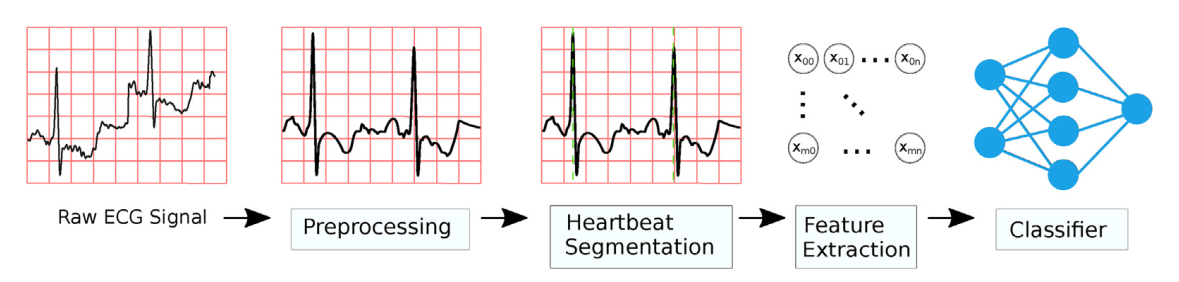
\includegraphics[width=15cm]{Figures/classifier.png}
\caption{مراحل اصلی یک سیستم خودکار تشخیص آریتمی\cite{Mondejar}}
\label{fig:classifierPicture}
\end{figure}
این روش در اکثر کارهای گذشته در زمینه‌ی تشخیص خودکار آریتمی به کار برده شده‌است. روش‌های متنوعی برای پیاده‌سازی الگوریتم دسته‌بندی استفاده شده‌اند، برای مثال در \cite{Exarchos2007} از سیستم‌های فازی\LTRfootnote{Fuzzy systems}، در \cite{deChazal2004} و \cite{Llamedo2011} از شبکه‌‌های عصبی مصنوعی\LTRfootnote{Artificial neural networks} و در \cite{Zhang2005} و \cite{Bazi2013} از ماشین‌های بردار پشتیبانی\LTRfootnote{Support Vector Machines (SVM)} برای دسته‌بندی انواع آریتمی استفاده شده‌است. در این پروژه نیز از همین معماری کلی استفاده کرده‌ایم، با این تفاوت که سعی شده‌است راه‌حلی برای بی‌درنگ ساختن این سیستم ارائه شود. 

همان‌طور که در بخش نیازمندی‌ها اشاره شد، بی‌درنگ بودن و قابل‌حمل‌بودن از نیازمندی‌های سیستم هستند. برای پاسخ‌گویی به این نیازمندی‌ها، اینترنت اشیا به عنوان راه‌حلی مناسب تشخیص‌ داده می‌شود، چرا که به کمک آن می‌توان بخشی از سیستم را بر روی دستگاهی ساده و قابل‌حمل، بدون نیاز به توان پردازشی بالا پیاده‌سازی کرده و پردازش‌های سنگین‌تر را به عهده‌ی یک سرور قرار داد. اینترنت اشیا ارتباط بین این بخش‌ها را ممکن می‌سازد.

سیستم بی‌درنگ پیاده‌سازی‌شده در این کار،  قادر به تشخیص نوع آریتمی هر یک از ضربان‌های گرفته‌شده از بیمار با دقتی بالا، و رساندن نتایج به کاربر است. در ادامه ابتدا به مفاهیم مورد استفاده در کار پرداخته و سپس روش طراحی و پیاده‌سازی سیستم تشخیص خودکار آریتمی و همین طور نتایج به دست آمده را شرح خواهیم‌داد. 
